\documentclass{article}
\usepackage[margin=1in]{geometry}
\usepackage{fancyvrb}
\usepackage{multicol}
\usepackage{hyperref}
\usepackage{amsmath}
\usepackage{amsfonts}

\usepackage[listings]{tcolorbox}

\definecolor{codegreen}{rgb}{0,0.6,0}
\definecolor{codegray}{rgb}{0.5,0.5,0.5}
\definecolor{codepurple}{rgb}{0.58,0,0.82}
\definecolor{backcolour}{rgb}{0.95,0.95,0.92}

\lstdefinestyle{mystyle}{
    language=Python,
    backgroundcolor=\color{backcolour},   
    commentstyle=\color{codegreen},
    keywordstyle=\color{magenta},
    numberstyle=\tiny\color{codegray},
    stringstyle=\color{codepurple},
    basicstyle=\ttfamily\footnotesize,
    breakatwhitespace=false,         
    breaklines=true,                 
    captionpos=b,                    
    keepspaces=true,                 
    numbers=left,                    
    numbersep=5pt,                  
    showspaces=false,                
    showstringspaces=false,
    showtabs=false,                  
    tabsize=2,
    escapechar=|,
    frame=single
}

\lstset{style=mystyle}

%\usepackage[T1]{fontenc}
\usepackage{tikz}
\usetikzlibrary{arrows.meta,
                calc, chains,
                decorations.pathreplacing,
                calligraphy,
                positioning,
                quotes,
                shapes}
                
\newcommand{\showfig}[2]{
\noindent\includegraphics[width=\textwidth]{#1}
\centerline{#1}
}
\newcommand{\bi}{\begin{itemize}}
\newcommand{\li}{\item}
\newcommand{\ei}{\end{itemize}}

\title{Linked List Bignums}
\author{CSCI 112, Lab 4}
\date{}

\begin{document}
\sloppy

\maketitle

\begin{description} 
\item[File names:]  Names of files, functions, and variables, 
when specified,
must be EXACTLY as specified.  This includes simple mistakes such
as capitalization.

\item[Individual work:]  All work must be your own.  Do not share
code with anyone other than the instructor and teaching assistants.
This includes looking over shoulders at screens with the code open.
You may discuss ideas, algorithms, approaches, {\em etc.} with
other students but NEVER actual code.  Do not use code
written by anyone else, in the class or from the internet.

\item[Documentation:] Each file should begin with a docstring
that includes your name, the class number and name, the lab
number, and  
a short description of the lab, as well as documentation pertinent
to that particular file.

\item[Addition and subtraction standard algorithm:]  You should be
familiar with the standard algorithms for addition and subtraction,
at least in base 10.  If you are not familiar with other number bases,
review them quickly here: \url{https://www.mathsisfun.com/numbers/bases.html}.

The standard subtraction and addition algorithms work fine in any
base.  You just have to remember that if you are in base 16, say,
and you ``borrow one'' from the next column, you are borrowing 16,
not 10.  Likewise, you ``carry one'' to the next column when you
get 16 or more, not 10.  Here are some worked examples to get
the hang of things:

Base 10 examples:\hfill
\begin{tabular}{rrrrr}
  &3 &9 &1 &5\\
$+$ &1 &2 &4 &5\\
\hline
  &5 &1 &6 &0\\
\end{tabular}\hfill
\begin{tabular}{rrrrr}
  &3 &9 &1 &5\\
$-$ &1 &2 &4 &5\\
\hline
  &2 &6 &7 &0\\
\end{tabular}

Base 8 examples:\hfill
\begin{tabular}{rrrrrr}
  &  &7 &5 &1 &3\\
$+$ &  &2 &3 &3 &5\\
\hline
  &1 &2 &0 &5 &0\\
\end{tabular}\hfill
\begin{tabular}{rrrrr}
  &7 &5 &1 &3\\
$-$ &2 &3 &3 &5\\
\hline
  &5 &1 &5 &6\\
\end{tabular}

Base 16 examples:\hfill
\begin{tabular}{rrrrr}
  &  &15 &4 &11\\
$+$ &  &4 &13 &13\\
\hline
  &1 &4 &2 &8\\
\end{tabular}\hfill
\begin{tabular}{rrrr}
  &15 &4 &11\\
$-$ &4 &13 &13\\
\hline
  &10 &6 &14\\
\end{tabular}

If you want more examples, just run my program {\tt arithmetic.py}
and paste the output into a new project on \url{https://www.overleaf.com}.

You can get easy base 8 and base 16 examples from python (remember that
in base 16 the digits 10 to 15 are: {\tt a, b, c, d, e, f}):
\begin{lstlisting}
>>> hex(0xaaa + 0x123)
'0xbcd'
>>> oct(0o666 + 0o123)
'0o1011'
\end{lstlisting}

\item[Bignums:]  Python has bignums (arbitrarily high integers) built in.  For example, Python
has no problem computing:
\begin{lstlisting}
>>> 1234567890987654321 * 1234567890987654321
1524157877457704723228166437789971041
\end{lstlisting}
Even though computers only natively support either 32 bit integers, or 64
bit integers.  Hence, the maximum integers supported in most programming
languages are either $2^{32} = 4.294.967.296$ or  $2^{64} = 18.446.744.073.709.551.616$.
Integers larger than this are supported in software.

When Python encounters integers that are too big for the 32 or 64 bit
registers, it automatically converts them to bignums.   Python's bignums
are implemented as dynamic arrays of digits in a large, fixed base.

In this lab we will build a Bignum class of our own that supports arbitrarily large integers
using linked lists.  Each cell in the linked list will hold a single position in
the base.  For example, if we choose base 10 for our bignums, each
cell in the linked list will hold a Python integer from 0 to 9.  If we choose
base 16 for our bignums, each cell in the linked list will hold a 
Python integer between 0 and 15.  If we choose 10,000 for our base,
each cell in the linked list will hold a Python integer between 0 and 9,999.

Here, for example, is a figure of what the number \lstinline{0o374} in base 8
looks like:

\begin{center}
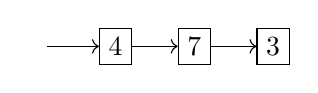
\begin{tikzpicture}
\tikzset{
  block/.style={draw, rectangle}
  }
\node[block] (A) {3};
\node[block,left of=A] (B) {7};
\node[block,left of=B] (C) {4};
\node[left of=C] (D) {};
\draw[->] (D) -- (C);
\draw[->] (C) -- (B);
\draw[->] (B) -- (A);
\end{tikzpicture}
\end{center}

Note that the smallest digit will be at the head of the list.  This will make arithmetic
much easier.

Make your Bignum class general, so it will support any base.  

Since there's no such thing as an ``empty'' bignum, we will not need the header
class used for linked lists in the book.  A bignum will hold the digit, the sign, and a 
pointer to the next bigger digit.

\item[Signs:]  Positive and negative numbers will be represented by
a separate field in the class called \lstinline{Bignum.sign}, with the value
of either plus or minus one.

\item[Initializing with Python ints:]  To make testing easy, Bignums will be initialized
by Python integers.  The initializing integer can be any size, of course,
using Python's native integers.  You will convert this to your linked list
representation of Bignums.  Here is the initializing routine for bignums
that you should use:
\begin{lstlisting}
    def __init__(self, n, base = 17):
        self.base = base
        if n < 0:
            self.sign = -1
        else:
            self.sign = 1
        self.n = abs(n)
        self.next = None
        self.overflow()
\end{lstlisting}
Needless to say, the \lstinline{Bignum.overflow} method will take care of
normalizing the integer to the range \lstinline{[0..(self.base-1)]} and
pushing any overflows (``carries'') along to the next cell in the list.

\item[Extracting Python ints:]
Also to make testing easy, include a \lstinline{Bignum.int} method that
converts your bignum into a Python int.  This will support easy testing
expressions such as:
\begin{lstlisting}
n = 2**100
self.assertEqual(n, Bignum(n).int())
\end{lstlisting}

\item[String method:]
While it will be nice to see the bignums converted to Python integers for 
testing, 
I find it easier to debug if I can see what the data structure looks like.
Build a \lstinline{__str__} method that shows the contents of bignums like this:
\begin{lstlisting}
>>> print(Bignum(20,8))
Bignum base 8: 4:2:+
>>> print(Bignum(20,2))
Bignum base 2: 0:0:1:0:1:+
>>> print(Bignum(-123,10))
Bignum base 10: 3:2:1:-
>>> print(Bignum(50,16))
Bignum base 16: 2:3:+
>>> 
\end{lstlisting}

\item[Addition and subtraction:]  Once you've got your Bignum class
working, 
implement the standard algorithms for addition and subtraction, as illustrated
above, to support the \lstinline{__add__} and \lstinline{__sub__} methods
for your Bignums.  

You will have to do a little sign checking at the beginning.  For example,
to subtract a negative number from a positive number, just convert the negative
to a positive and then add.  Or, for another example, 
to subtract a larger number, $a$, from a smaller number, $b$, use the formula:
\[
b - a = -(a - b)
\]
So you will always be subtracting the smaller from the larger.   There are a few
other cases for you to work out: each operand can be positive or negative,
and either one could be the larger.  There should be eight cases in all, then, right?

\item[Leading zeros:]  Some operatrions may result in leading zeros, for example,
$12345 - 12300$ in base 10.  Your Bignum class should clean up any result
by removing these unecessary zeros.

\begin{lstlisting}
>>> print(Bignum(123456, 10) - Bignum(123000, 10))
Bignum base 10: 6:5:4:+
>>> 
\end{lstlisting}


\item[Recursion:]  Note, if you use recursion in your bignum calculations,
you may run into recursion depth limits with very large numbers.
This will not be considered a bug.

\item[Calculator:] Use your infix calculator from the previous lab to
make a Bignum calculator!

\item[Turn in:] Files {\tt bignum.py} and {\tt bignum\_test.py} in folder
{\tt csci112lab04yourname}, zipped and turned into Canvas.

\item[Optional additions:] ~

\begin{itemize}
\item
Multiplication can be done with the standard algorithm, or using the following facts:
\[
ab = 
\left\{\begin{array}{ll}
0 & \mbox{if $b=0$} \\
a+a(b-1) & \mbox{if $b$ is odd} \\
2(a(b/2)) & \mbox{if $b$ is even}
\end{array}\right.
\]
You will have to implement a divide by 2 function, but the rest can be done
with recursion and addition.

\item Division, exponentiation, {\em etc.}

\item Run some experiments to see how the timing of your
Bignums changes with the size of the base.  Note that Python will
not use native integers if the size of the integer is greater 
than the size of a native integer.  Since your calculations can result
in numbers in the cells up to 2(base), or base$^2$ if you do multiplication, 
your base should probably
not exceed $2^{16}$ for 32 bit computers, or $2^{32}$ for 64 bit
computers.  (Why?)

Once you find the best base for your implementation, compare
times on your implementation with those for native Python bignums.
How much slower are you?  Do you think it makes a big-O difference,
or not?  Why?  Can you prove it with some data?

Write up your experiments and conclustions in a short document.

    
\end{itemize}

\newpage
\item[My implementation headers:]   
You do not have to follow my implementation here, 
but in my Bignum class 
I used the following approach.  Some of my functions are recursive,
and some are iterative.

I have also supplied my unit test file, as a start, for yours.

\begin{lstlisting}
def __init__(self, n, base = 17):
def __str__(self):
def int(self):
    '''convert to Python integer'''
def copy(self, end=None):
def add(self, other):
    '''add absolute values'''
def __add__(self, other):
    '''figure out signs, then add or sub and fix result'''
def sub(self, other):
    '''subtract absolute values, if self < other return negative of other-self'''
def __sub__(self, other):
    '''figure out signs then add or sub and fix result'''
def cmp(self, other):
    '''compare absolute values, return -1,0,1 for less, equal, greater'''        
def __lt__(self, other):
    '''less than, using signs and cmp'''
def __eq__(self, other):
    '''equality, using signs and cmp, needed for unit tests'''
def remove_zeros(self):
    '''remove leading zeros'''               
 def inc_next(self, amt=1):
    ''if amt > 0 'increment the next cell.  if absent, create it'''
def overflow(self):
    '''any cell that is larger than the base is reduced and carried to the next cell''' 
def dec_next(self, amt=1):
    '''if amt > 0 decrement next cell, if absent, raise error'''            
def underflow(self):
    '''any cell that is less than 0 is incremented by borrowing from the next'''
\end{lstlisting}
\end{description}



\end{document}
